\chapter{The Helmholtz Problem}

\section{Good Cop vs. Bad Cop}

Solving the general Helmholtz equation,
\begin{equation}
-\Delta u + k^2 u = f,
\end{equation}
with numerical methods, and particularly multigrid methods, is an open problem \cite{Ernst2012}.  We will briefly touch upon why this is in this section before moving forward with the formulation used in this project.  For simplicity, we consider only the cases where $k^2=+1$ and $k^2=-1$, respectively referred to as "Good Cop" and "Bad Cop" Helmholtz equations.  First, we introduce the concepts of \textit{positive definite} and \textit{negative definite} matrices.


\textbf{Def 2.1} A $n \times n$ Hermitian matrix, $A$, is said to be \textbf{positive definite} if the scalar $z^* A z$ is \textit{positive} for all real, non-zero column vectors $z$ of size $n$.  Here, $z^*$ denotes the conjugate transpose of the vector $z$.  If however $z^* A z$ is \textit{negative}, then $A$ is called a \textbf{negative definite} matrix.  Lastly, if $z^* A z$ can be either \textit{positive} or \textit{zero}, then it is called \textbf{positive semi-definite}, and, similarly, if $z^* A z$ can be either \textit{negative} or \textit{zero}, it is called \textbf{negative semi-definite} \cite{Keener2000}.


It is worth noting that the existence of positive, negative or zero eigenvalues of a matrix can also be used to define what type of matrix $A$ is.  Since we strive to convert our initial equation formulation $-\Delta u + k^2 u = f$, also called the \textit{strong form}, to a linear system $Au=f$, we can extend (2.1) to the strong form of our equations where $A=-\Delta + k^2$.  Furthermore, in numerical methods, a positive definite operators are highly desirably as they can be easily inverted and contain other useful properties.

The negative Laplacian operator, $-\Delta$, is well known for being a positive definite operator.  Therefore, the positive definiteness of the Helmholtz equation is dependent on the $k^2$ term.  If $k^2 \geq 0$, i.e. the "Good Cop" form, then the equation remains positive definite and is solvable with common methods.  However, if $k^2 \leq 0$, i.e. the "Bad Cop" form, then the equation becomes indefinite and solution becomes much trickier.  As stated at the beginning of this section, solving the indefinite form of the Helmholtz equation is still an open research topic of interest.

\section{Variational Formulation}
For the reasons given in the previous section, we will derive the variational form for the case where $k^2=+1$, or the "Good Cop" Helmholtz equation \cite{Farrell2018},
\begin{align}
-\Delta u + u &= f \;\; in \;\; \Omega, \\
u &= u_0 \;\; on \;\; \Gamma_D \subset \partial \Omega, \\
\nabla u\cdot n &= g \;\; on \;\; \Gamma_N \subset \partial \Omega.
\label{pde}
\end{align}
This decision is mostly arbitrary at this stage because the sign can be easily flipped later to switch between the "Good Cop" and "Bad Cop" equations.  To discretize this equation, we use the same finite elements method that we used for the poisson equation. We start by multiplying by a test function $v$ and integrating over the domain to obtain,
\begin{equation}
-\int_{\Omega} (\Delta u) \, v \, dx + \int_{\Omega} u \, v \, dx = \int_{\Omega} f \, v \, dx.
\end{equation}
Applying integration by parts to the Helmholtz equation gives,
\begin{equation}
\int_{\Omega} \nabla u \cdot \nabla v \, dx - \int_{\Gamma_N} v \, (\nabla u \cdot n) \, ds + \int_{\Omega} u \, v \, dx = \int_{\Omega} f \, v \, dx.
\end{equation}

We assume the test function $v$ again vanishes on the parts of the boundary where the solution $u$ is known which simplifies the weak form to,
\begin{equation}
\int_{\Omega} \nabla u \cdot \nabla v \, dx + \int_{\Omega} u \, v \, dx = \int_{\Omega} f \, v \, dx.
\end{equation}
We use the test and trial spaces defined in \eqref{TrialSpace} and \eqref{TestSpace}, and define the discrete form of $u$, $u_h \in V_h \subset V$ and plug it back into the variational formulation which gives the discretretized weak form,
\begin{equation}
\int_{\Omega} \nabla u_h \cdot \nabla v \, dx + \int_{\Omega} u_h \, v \, dx = \int_{\Omega} f \, v \, dx \;\; \forall v \in \hat{V_h} \subset \hat{V}.
\end{equation}
Plugging the ansatz \eqref{ansatz} for $u_h$ the bases into the variational form gives,
\begin{equation}
\sum^N_{j=1} U_j \int_{\Omega} \nabla \phi_j \cdot \nabla \phi_i \, dx + \sum^N_{j=1} U_j \int_{\Omega} \phi_j \, \phi_i \, dx = \int_{\Omega} f \, \phi_i \, dx \;\;\; i = 1,2,...,N.
\end{equation}

Therefore, the linear system for the "Good Cop" Helmholtz equation is,
\begin{equation}
A U = b
\end{equation}
where,
\begin{align}
A_{ij} &= \int_{\Omega} \nabla \phi_j \cdot \nabla \phi_i \, dx + \int_{\Omega} \phi_j \, \phi_i \, dx \\
b_i &= \int_{\Omega} f \, \phi_i \, dx.
\end{align}

\section{Method of Manufactured Solutions}

As described above, we will use the \textit{Method of Manufactured Solutions} to verify our formulation and solver.  We choose our exact solution to be,
\begin{equation}
u_e(x,y) = 1 + x^2 + 2 y^2.
\end{equation}
Inserting $u_e$ into equation \eqref{pde} we find that $u_e$ is a solution if,
\begin{align}
f(x,y) &= -6 + 1 + x^2 + 2 y^2, \\
      &= -5 + x^2 + 2 y^2, \, and \\
u_0(x,y) &= 1 + x^2 + 2 y^2.
\end{align}
We also choose the domain to be,
\begin{equation}
\Omega = [0,1] \times [0,1].
\end{equation}
\begin{figure}[!ht]
\begin{center}
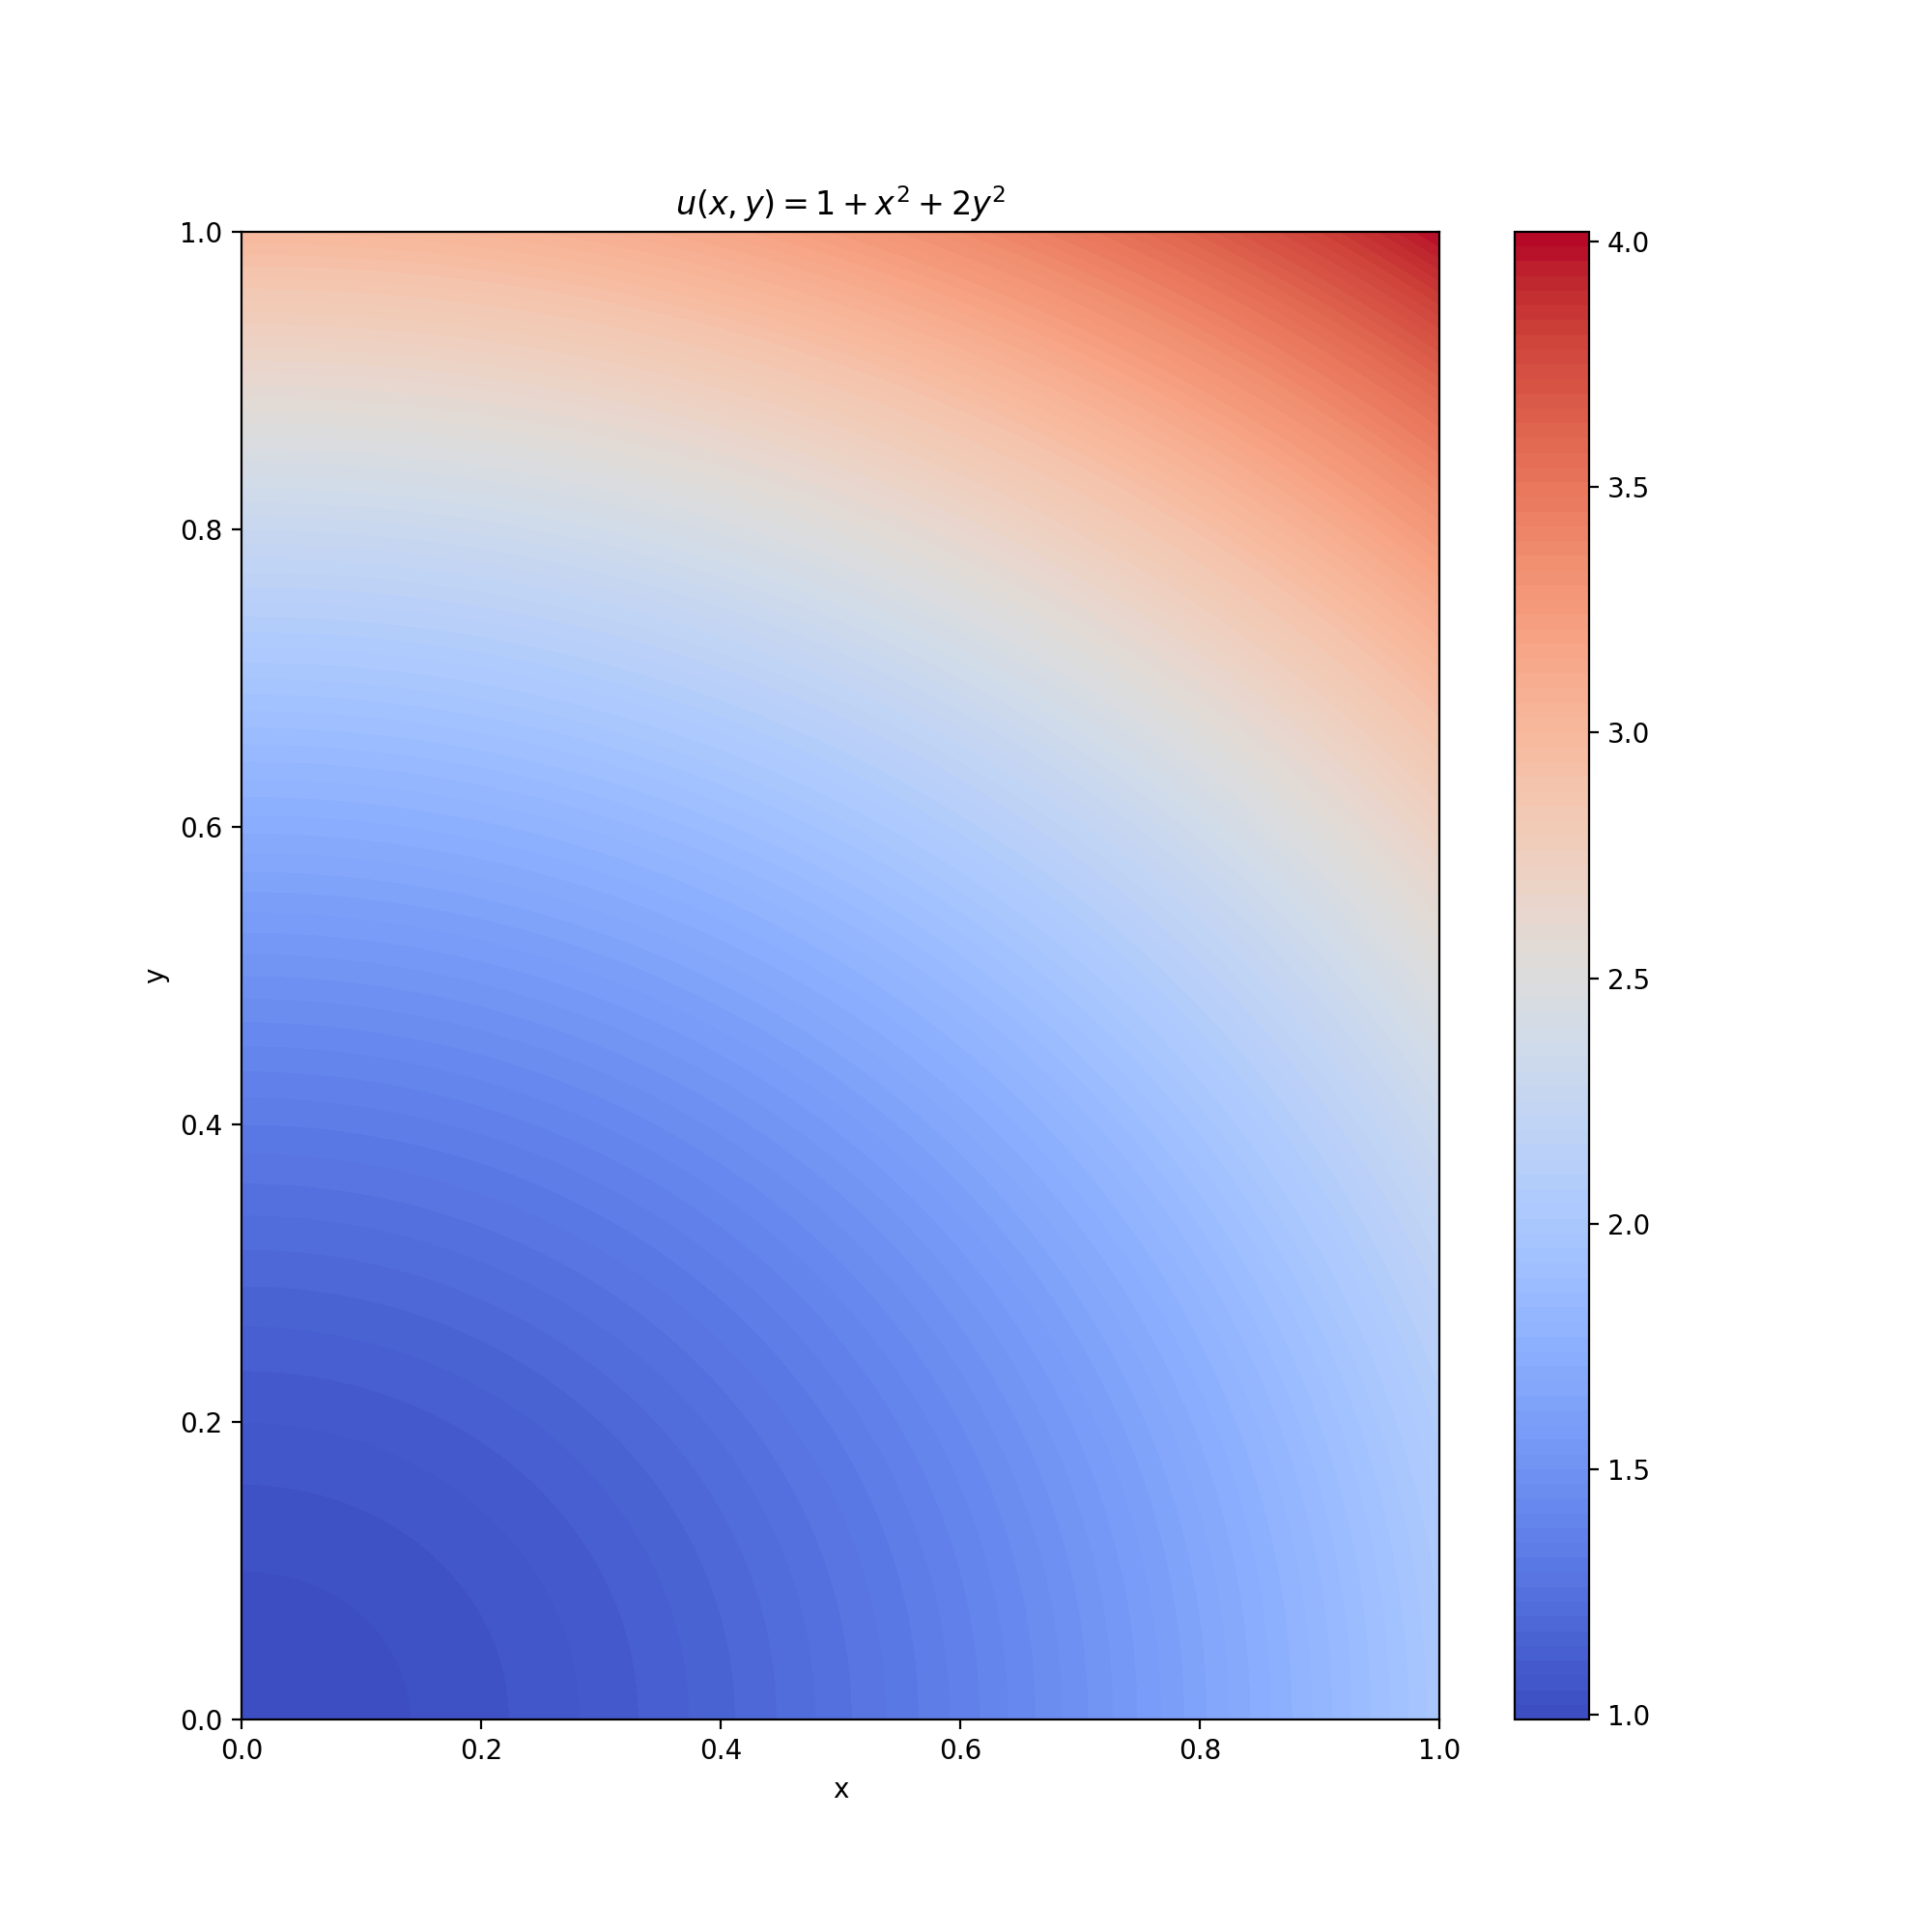
\includegraphics[scale=0.4]{figures/Quad_Exact.png}
\end{center}
\caption{Quadratic exact solution.}
\label{QuadExact}
\end{figure}


\subsection{PETSc Formulation}

In PETSc, the \textit{primal problem} is set by the functions PetscDSSetExactSolution, PetscDSSetResidual and PetscDSSetJacobian.  Each function requires a specific equation form as the inputs.  The residual function is requires the form,
\begin{equation}
\int_\Omega \phi_i f_0(u, u_t, \nabla u, x, t) + \nabla\phi_i \cdot {\vec f}_1(u, u_t, \nabla u, x, t),
\end{equation}
and the jacobian function takes the form,
\begin{equation}
\begin{split}
\int_\Omega &\phi_i g_0(u, u_t, \nabla u, x, t) \phi_j + \\
&\phi_i {\vec g}_1(u, u_t, \nabla u, x, t) \nabla \phi_j + \\
&\nabla\phi_i \cdot {\vec g}_2(u, u_t, \nabla u, x, t) \phi_j + \\
&\nabla\phi_i \cdot {\overleftrightarrow g}_3(u, u_t, \nabla u, x, t) \cdot \nabla \phi_k.
\end{split}
\end{equation}
Therefore, in the multigrid code we use the function inputs,
\begin{align}
f_0 &= u - (-5 + x^2 + 2 y^2), \\
f_1 &= \nabla u, \\
g_0 &= 1.0, \\
g_1 &= 0.0, \\
g_2 &= 0.0,\; and \\
g_3 &= 1.0.
\end{align}

\subsection{Trigonometric MMS}

To test more complex finite elements, an exact solution comprised of trigonometric functions is needed.  Therefore, we choose the exact solution,
\begin{equation}
u_e^{trig}(x,y) = sin( 2 \pi x) + sin( 2 \pi y).
\end{equation}
Inserting $u_e^{trig}$ into equation \eqref{pde} we find that $u_e$ is a solution if,
\begin{align}
f(x,y) = 4 \pi^2 sin(2 \pi x) +& 4 \pi^2 sin(2 \pi y) + sin( 2 \pi x) + sin( 2 \pi y), \, and \\
u_0(x,y) &= sin( 2 \pi x) + sin( 2 \pi y).
\end{align}
\begin{figure}[!ht]
\begin{center}
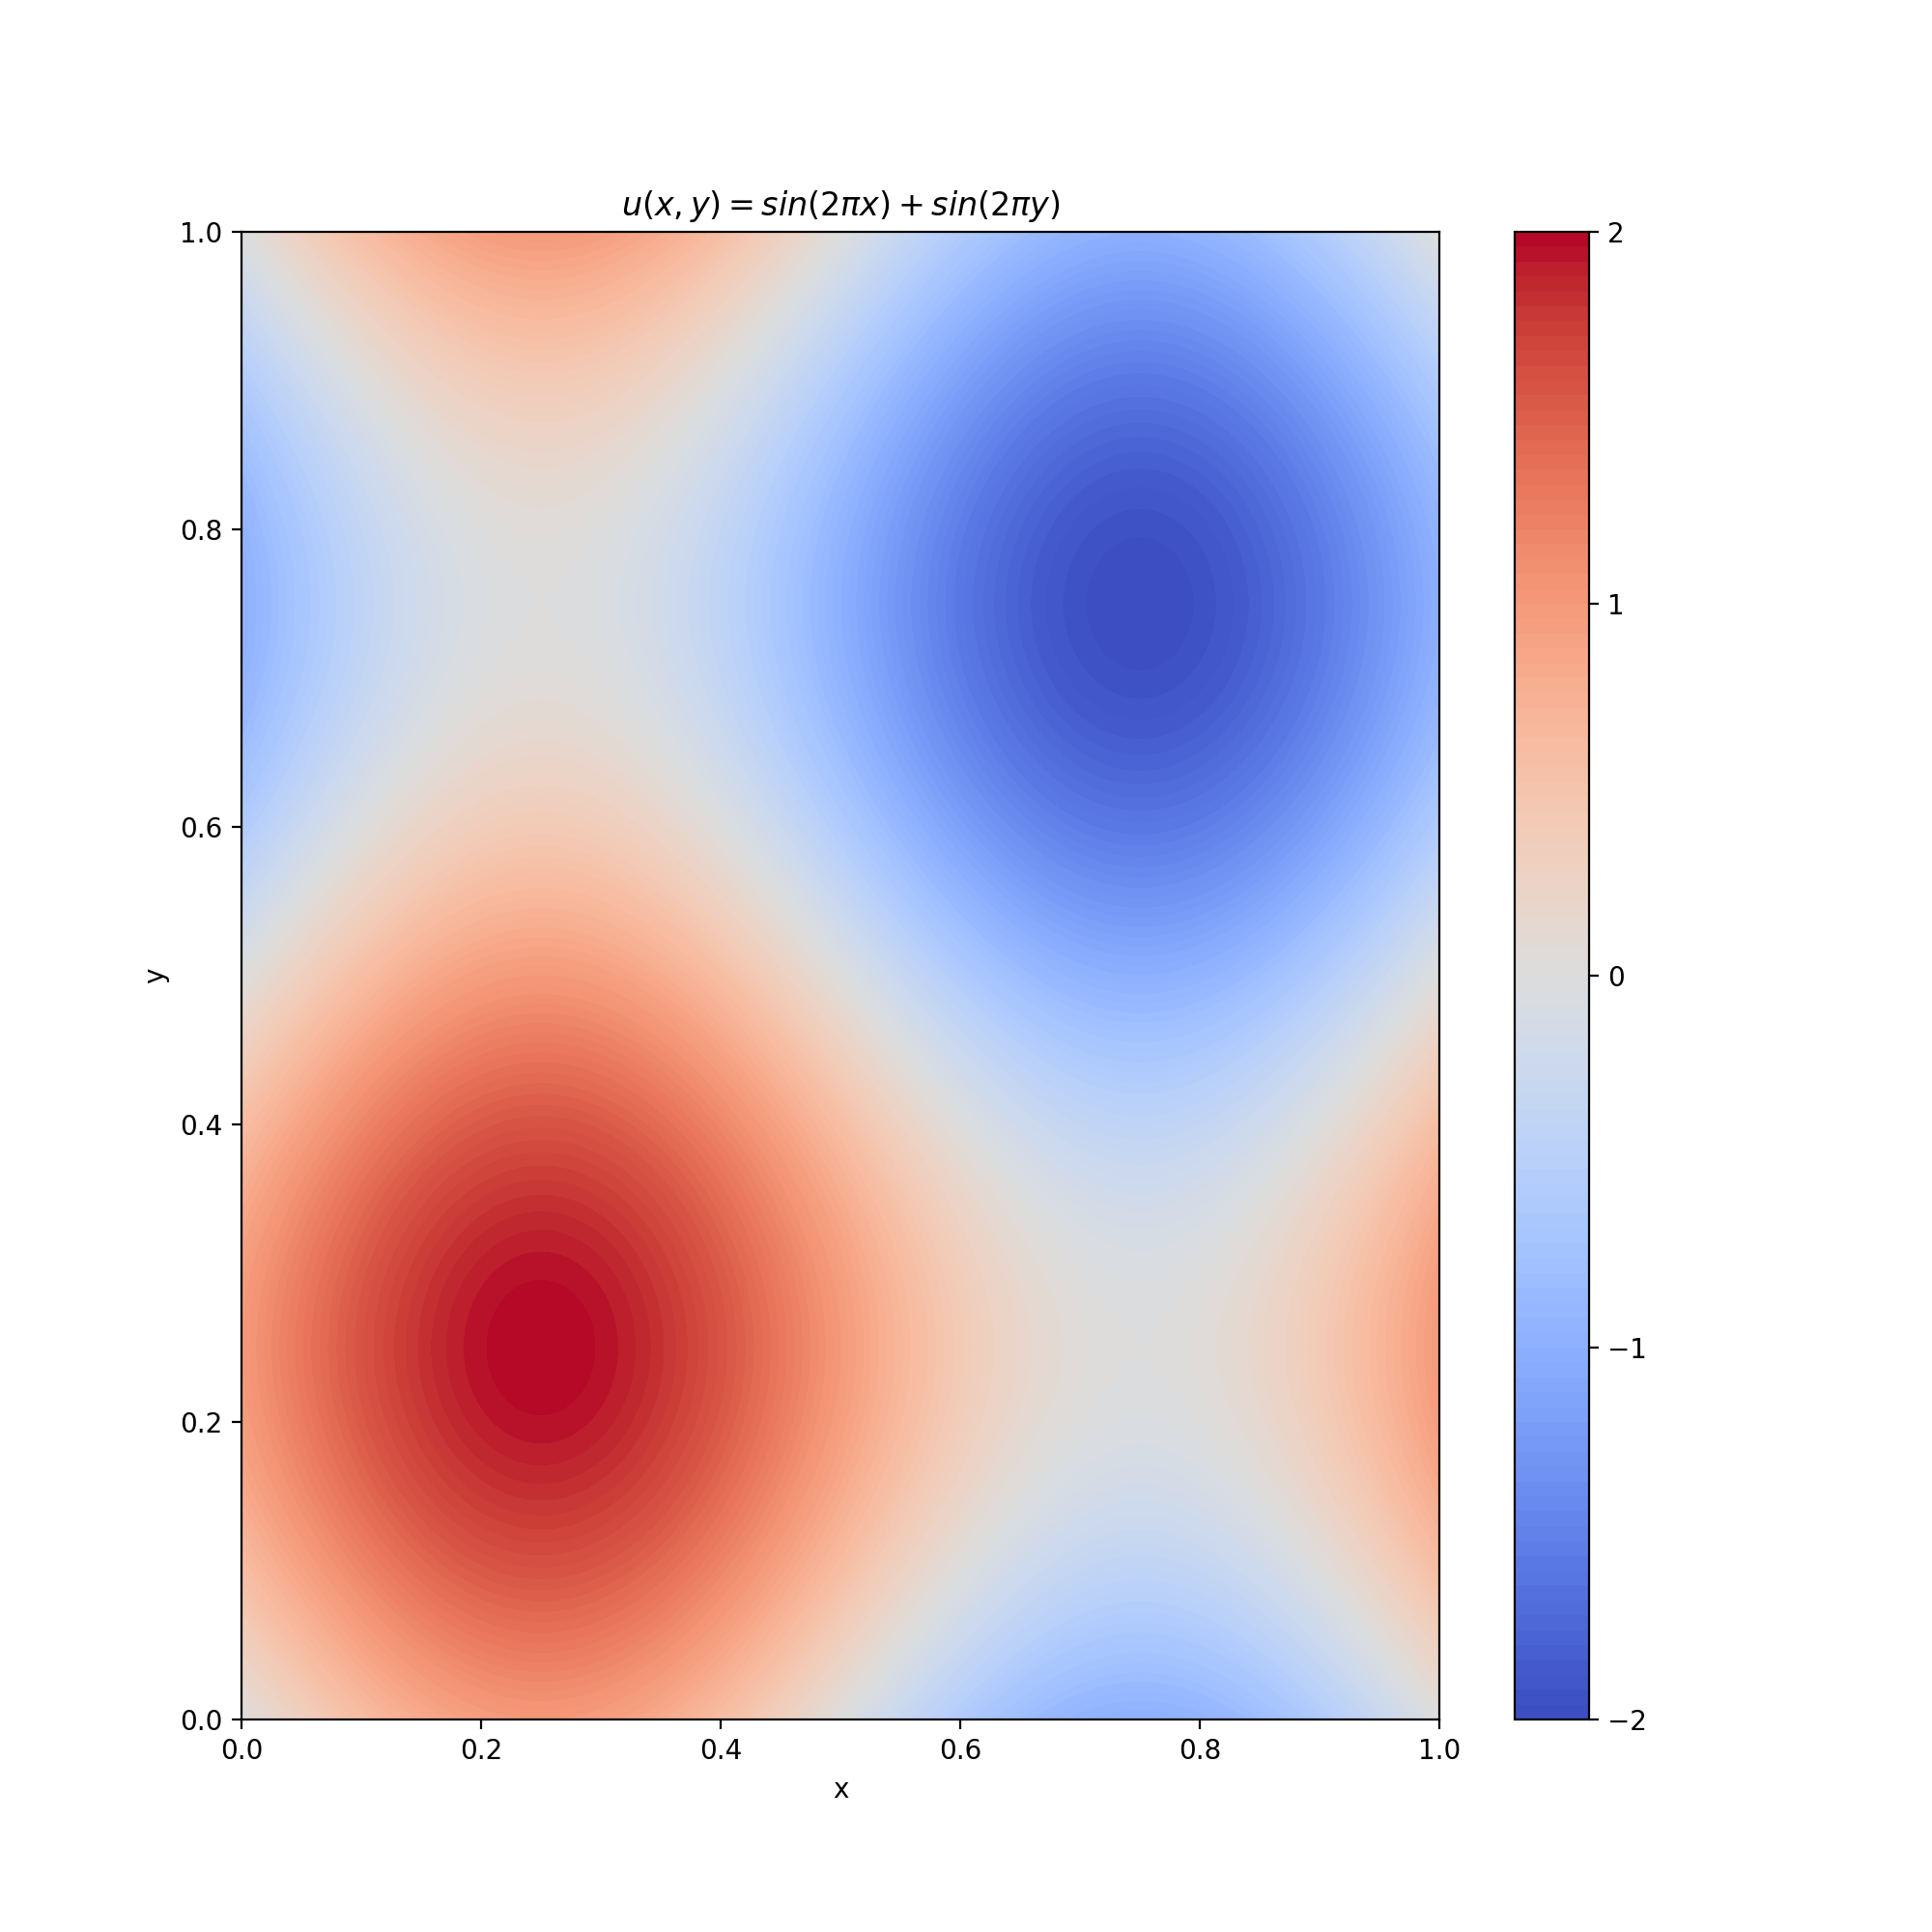
\includegraphics[scale=0.4]{figures/Trig_Exact.png}
\end{center}
\caption{Trigonometric exact solution.}
\label{TrigExact}
\end{figure}

\subsection{Trigonometric PETSc Formulation}

For the trigonometric case, the residual and jacobian inputs are,
\begin{align}
f_0 &= u - (4 \pi^2 sin(2 \pi x) + 4 \pi^2 sin(2 \pi y) + sin( 2 \pi x) + sin( 2 \pi y)), \\
f_1 &= \nabla u, \\
g_0 &= 1.0, \\
g_1 &= 0.0, \\
g_2 &= 0.0,\; and \\
g_3 &= 1.0.
\end{align}
